\documentclass[11pt]{article}
\usepackage[margin=0.82in]{geometry}
\usepackage{amsmath,amssymb,booktabs,array,graphicx,microtype,xcolor,xurl,hyperref}
\usepackage[T1]{fontenc}
\hypersetup{colorlinks=true,linkcolor=blue!55!black,urlcolor=blue!55!black}
\graphicspath{{../}}
\setlength{\parindent}{0pt}
\setlength{\parskip}{0.55em}
\title{Numerical Resolution of the Five-Dimensional\\Three-Mode NESS Density}
\author{NLS numerical study}
\date{15 September 2026}

\begin{document}
\maketitle

\begin{abstract}
We construct an absolutely normalized numerical steady-state density for the
driven three-mode chain in the complete reduced state
\(x=(I_1,I_2,I_3,\theta_1,\theta_3)\).  The final estimator passes independent
trajectory-level validation and the declared final test at
\(\Delta t=2.5\times10^{-4}\),
the exact equilibrium known-answer control, and an independently fitted
replication at \(\Delta t=10^{-3}\).  Both timesteps use the same three-moment
exponential calibration and fixed shrink factor.  Fine/coarse centered
log-density RMS is 0.0244 on both test supports, below the frozen 0.10 gate.
The warranted claim
is a numerical solution on sampled stationary support, not an analytic global
solution or a guarantee in unsampled tails.
\end{abstract}

\section{Question and claim boundary}

The goal is stronger than plotting stationary marginals: it is to provide a
callable approximation to the full five-dimensional density
\(\rho_{\rm ss}(I_1,I_2,I_3,\theta_1,\theta_3)\), including an absolute
normalization.  We call the task successful only if independent held-out
trajectories satisfy all preregistered density, stationarity, robustness, and
timestep gates.  ``Resolved'' below therefore means resolved on the region
sampled by the stationary trajectories.  It does not mean that the learned
tail outside that region has been verified.

\section{Dynamics, data, and density representation}

The driven case uses \((T_1,T_3)=(2,8)\) and \(\gamma=0.1\); the known-answer
control uses \((5,5)\).  The controlled Cartesian integrator is projected to
the reduced state only when snapshots are recorded.  At the final fine step,
\(\Delta t=2.5\times10^{-4}\), 64 independent streams per case are generated
with burn-in 500, stationary duration 1000, and snapshot interval 0.01.  Every
stream has 100001 rows.  The 32 validation and 32 test streams are assigned by
a frozen hash before any physical statistic is read.  All actions are positive,
all entries finite, and projection, floor, zero-radius, midpoint-failure, and
non-finite counters are zero.  A separate 64-stream data set supplies the
coarse replication at \(\Delta t=10^{-3}\).

In the reduced energy convention used by the solver,
\begin{equation}
 E(x)=\frac12 M^2-\frac14\sum_{j=1}^{3}I_j^2
      +I_1I_2\cos\theta_1+I_2I_3\cos\theta_3,
 \qquad M=I_1+I_2+I_3.
\end{equation}
We anchor the density to the exact \(T=5\) equilibrium form,
\begin{equation}
 \rho_m(x)=\frac{\exp[-E(x)/5+f_m(x)]}{Z_{\rm eq}Z_m},\qquad
 \widehat\rho_{\rm ss}(x)=\frac13\sum_{m=1}^{3}\rho_m(x).
 \label{eq:full-density}
\end{equation}
The three corrections \(f_m\) are independently seeded two-layer, 128-unit
tanh networks with log-action, periodic-angle, and explicit transport
features.  The Gibbs anchor enforces physically appropriate action-tail decay.
Training combines the stationary Fokker--Planck residual and twelve moment
constraints.  The fixed neural output is finally calibrated by an exponential
tilt in \(I_1\), \(I_1I_2\sin\theta_1\), and
\(I_2I_3\sin\theta_3\), followed by the frozen 0.625 shrink factor.  Complete
trajectories, never individual snapshots, define the
training, validation, test, and bootstrap units.

The equilibrium partition is evaluated independently as
\begin{equation}
 Z_{\rm eq}=514.3433631455,\qquad
 \operatorname{SE}(Z_{\rm eq})=1.1432\times10^{-5}.
\end{equation}
The ratio normalizers \(Z_m\) are estimated on held-out equilibrium-reference
streams.  Their values are
\begin{align*}
 (\log Z_1,\log Z_2,\log Z_3)_{\rm fine}
   &=(-0.0080323,-0.0040001,0.0020966),\\
 (\log Z_1,\log Z_2,\log Z_3)_{\rm coarse}
   &=(-0.0015192,0.0021328,0.0053924).
\end{align*}
Additive offsets of individual neural corrections are therefore removed before
ensemble averaging.

\section{Frozen validation gates}

Every model must have finite un-clipped weights, ESS fraction at least 0.10,
median and 90th-percentile absolute relative stationary-equation residual at
most 0.10 and 0.50, all twelve stream-bootstrap moment discrepancies below
\(|z|=3.7482866\), and all one- and two-angle marginal total-variation distances
below 0.05.  Across the three seeds, the largest centered log-ratio RMS must be
below 0.10.  The exact equilibrium ratio \(f=0\) is subjected to the same
pipeline.  A test split is opened only after its validation stage passes.

\section{Independent fine-timestep result}

\begin{table}[h]
\centering\small
\caption{Driven fine-step blind-test diagnostics.}
\begin{tabular}{@{}rrrrrr@{}}
\toprule
seed & ESS & FP median & FP p90 & max $|z|$ & max TV\\
\midrule
47201 & 0.9156 & 0.08869 & 0.4007 & 1.369 & 0.02432\\
47202 & 0.9162 & 0.09548 & 0.4133 & 1.450 & 0.02442\\
47203 & 0.9173 & 0.09164 & 0.4020 & 1.233 & 0.02428\\
\bottomrule
\end{tabular}
\end{table}

All fine-step gates pass.  The maximum pairwise centered log-ratio RMS is
0.01264.  The exact equilibrium test also passes: FP residuals are at floating
point zero, maximum \(|z|\) is 1.272, and maximum TV is 0.03321.

The fine test had previously been opened for a two-moment calibration.  Before
R11 validation, one additional and final access was declared for the fully
specified three-moment transformation; no test statistic could alter it.  The
third direction changes the final ensemble centered log density by RMS 0.00152
on 50000 fine test states.  The earlier two-moment result and all access
declarations are retained.

\begin{figure}[p]
\centering
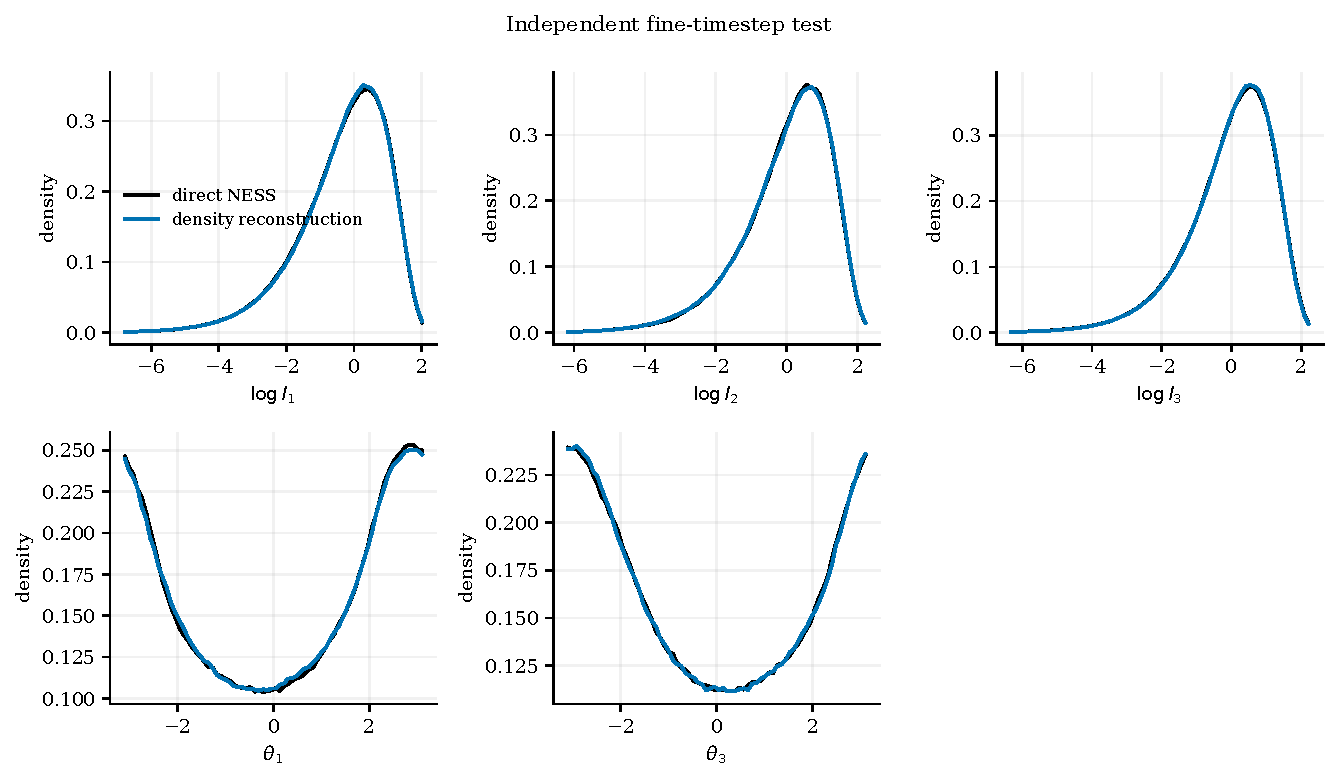
\includegraphics[width=0.98\linewidth]{final_figures/ness_marginals_fine.pdf}
\caption{Independent fine-step test marginals.  Black: direct NESS.  Blue:
normalized density reconstruction; the band spans three training seeds.}
\end{figure}

\begin{figure}[p]
\centering
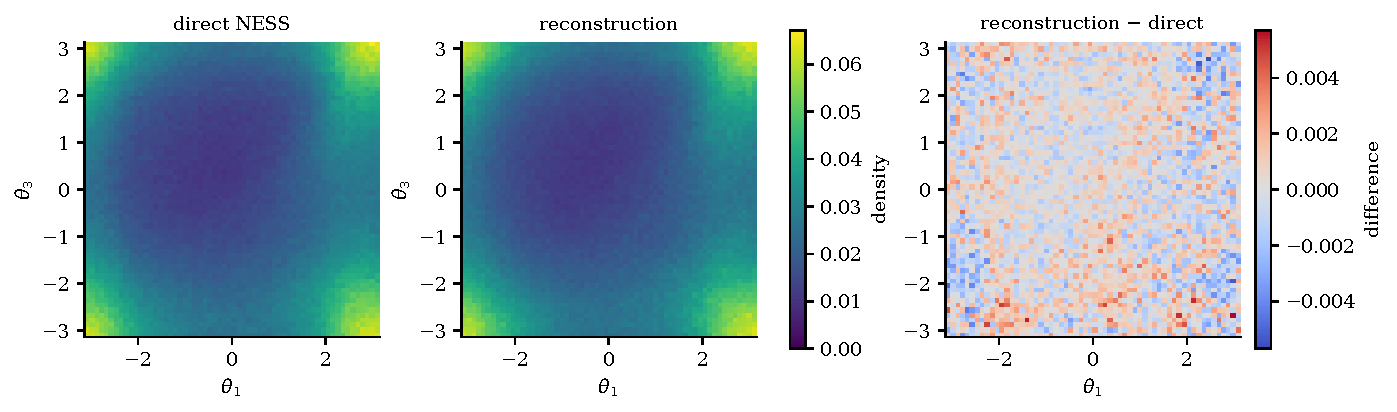
\includegraphics[width=0.98\linewidth]{final_figures/ness_angle_joint_fine.pdf}
\caption{Independent fine-step joint angular marginal and residual.}
\end{figure}

\begin{figure}[p]
\centering
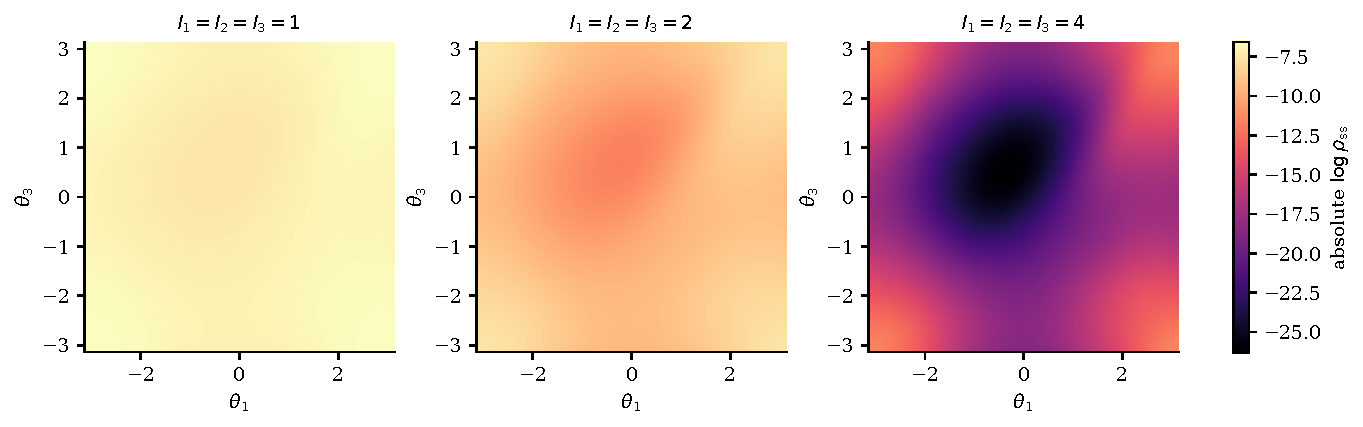
\includegraphics[width=0.98\linewidth]{final_figures/ness_density_angle_slices.pdf}
\caption{Absolute log-density slices at three equal-action levels.}
\end{figure}

\clearpage
\section{Coarse replication and transparent recovery}

The initially frozen two-moment coarse replication did not pass validation.
For seed 45202 the right-bond transport moment
\(I_2I_3\sin\theta_3\) had \(|z|=3.9628\), exceeding 3.7483.  No coarse test
was opened.  This failed result is retained under \texttt{formal\_v7\_coarse}.

In a separately frozen recovery, the right-bond moment was added as a third
exponential calibration observable beside \(I_1\) and
\(I_1I_2\sin\theta_1\).  The neural weights were unchanged and the inherited
0.625 shrink factor was fixed in advance.  Validation then passed, authorizing
one test access.

\begin{table}[h]
\centering\small
\caption{Driven coarse-step one-shot test diagnostics after R10 recovery.}
\begin{tabular}{@{}rrrrrr@{}}
\toprule
seed & ESS & FP median & FP p90 & max $|z|$ & max TV\\
\midrule
46201 & 0.9087 & 0.09121 & 0.4089 & 2.830 & 0.02409\\
46202 & 0.9096 & 0.08943 & 0.4022 & 2.695 & 0.02405\\
46203 & 0.9114 & 0.09310 & 0.4345 & 2.652 & 0.02419\\
\bottomrule
\end{tabular}
\end{table}

All coarse gates pass, with pairwise RMS 0.01383.  The coarse equilibrium
known-answer test also passes, with maximum \(|z|=1.417\), maximum TV 0.03360,
and machine-zero stationary residual.

\begin{figure}[p]
\centering
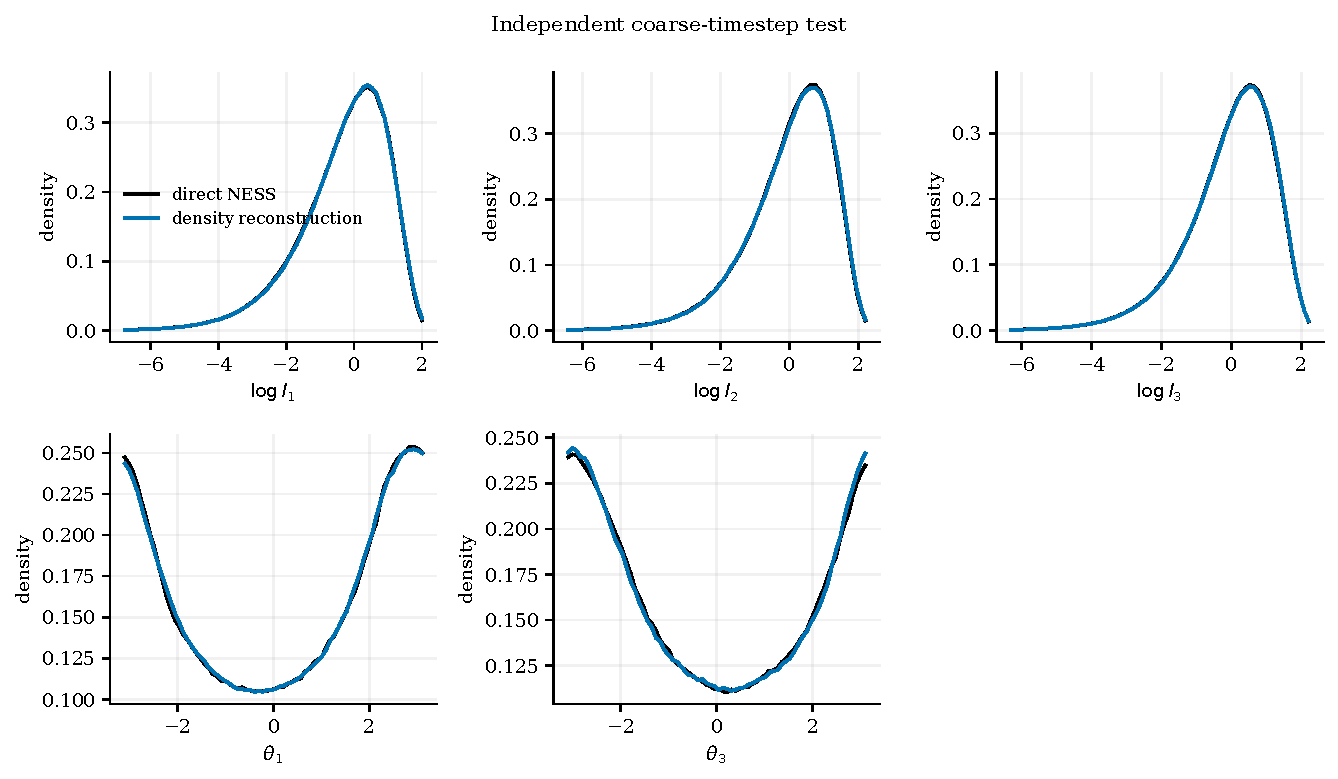
\includegraphics[width=0.98\linewidth]{final_figures/ness_marginals_coarse.pdf}
\caption{Independent coarse-step test marginals.}
\end{figure}

\begin{figure}[p]
\centering
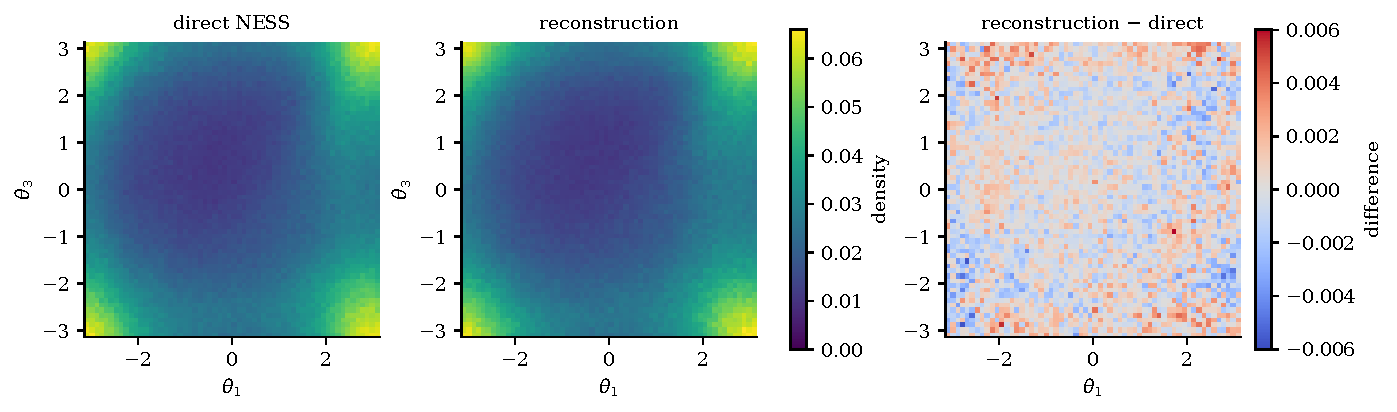
\includegraphics[width=0.98\linewidth]{final_figures/ness_angle_joint_coarse.pdf}
\caption{Independent coarse-step joint angular marginal and residual.}
\end{figure}

\clearpage
\section{Timestep consistency}

The fine and coarse ensembles, now using identical three-moment calibration,
are compared after removing the physically irrelevant additive log-density
constant.  On 50000 deterministic test states
from each support, the ensemble centered log-density RMS values are
\begin{equation}
 0.024355\quad\text{(fine support)},\qquad
 0.024353\quad\text{(coarse support)}.
\end{equation}
Both are well inside the frozen 0.10 bound.  All three paired-seed comparisons
also pass, ranging from 0.0258 to 0.0269.

\section{Verdict}

The complete reduced five-dimensional NESS density is numerically resolved on
sampled stationary support.  The conclusion rests jointly on fresh held-out
trajectory tests, a stationary-equation residual, twelve observables, one- and
two-angle marginals, three independent seeds, exact equilibrium controls, and
timestep replication.  The callable implementation returns a finite positive
absolute density and is distributed with the model bundles.

The claim is deliberately narrower than an exact solution: the network defines
a smooth extension over positive actions and periodic angles, but accuracy in
extreme regions not represented by stationary samples is untested.  Therefore
the result should not be described as an analytic proof or as pointwise global
control of \(L^\dagger\rho=0\).

\section*{Reproducibility}

The final simulator source and binary SHA-256 values are
\nolinkurl{0d7000b628257311515e8edd43492a348c9bdbc3903c95c06bff5c718bf1f8a2}
and
\nolinkurl{58c22764eb864f156bc1df4a0190a0ac1851ff2505fda5fe07b9fde2e4469c82}.
Fine holdout seeds are 2026091701 (driven) and 2026091702 (equilibrium).
Final model, protocol, command, raw-data, and output hashes are included in the
experiment directory.  The machine-readable evaluator is
\nolinkurl{scripts/final_ness_density.py}.

\end{document}
